\chapter{Einleitung}
Die Astrophysik zeichnet aus, dass im Gegensatz zu Laborexpermienten, diese ihre Observablen nicht gezielt beeinflussen können.
Somit sind sie angewiesen die begrenzten kosmischen Experimente ihre Zeit passiv zu beobachten. 
Dabei übernimmt das FACT Teleskope die Aufgabe mehrere kosmische Strahlungsquellen zu beobachten und bei Anormalitäten größere Teleskope, für genauere Observation von Ereignissen, zu informieren. 

Im Feld der Astroteilchen Physik werden verschiedene Quellen im Weltraum observiert.
Ziel der Observation ist ein tiefgreifendes Verständiniss über die Entstehung sowie die dominierenden Wechselwikungsprozesse zu erlangen. 
Quellen komsicher Strahlung sind überwiegend aktive galaktische Kerne, Neutronensterne und Supernova-Überreste. 
Die Energie der Teilchen decken ein Spektrum von \SI{e7}{\electronvolt} bei solarer kosmischen Strahlung bis zu \SI{e20}{\electronvolt} bei extragalaktischer kosmischen Strahlung ab. 

\begin{figure}
  \centering
  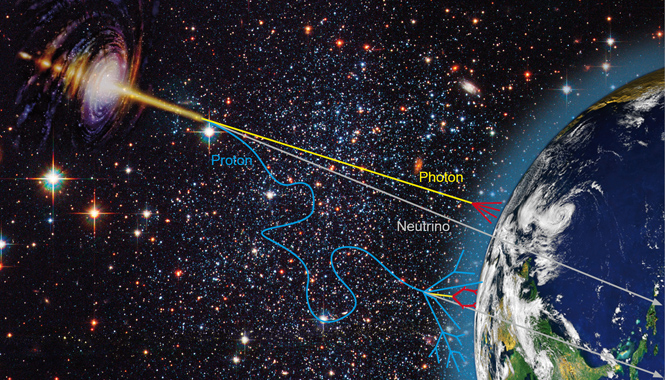
\includegraphics[width=0.6\textwidth]{./images/sources-detection.jpg}
  \caption{Way form source to detection~\cite{overview-detec}}
\end{figure}

Bei ihrem Weg von der Quelle durchs Universum treffen auf die Atmosphäre der Erde durchschnittlich \SI{1e5}{\per\second\per\meter\squared} Teilchen.
Diese produzieren je nach Teilchenart und Energie weitere Schauer, in denen viele weitere sekundär Teilchen erzeugt werden. 
Je nach Teilchenart gibt es verschiedene Detektionsmöglichkeiten, wovon das FACT eine erdbasierte Variante für \gamma-Quanten und Hadronen ist. 
Die verschiedenen kosmischen Teilchen lassen sich in drei verschiedenen Klassen einteilen. 
Dabei zählt der Sonnenwind zu einer der ständigen Quellen durch die geladene kosmische Strahlung auf die Erdatmosphäre trifft.


\section{Neutrinos}
Aufgrund ihrer elektrischen Neutralität sowie ihres geringen Wirkungsquerschnitts liefern Neutrinos Informationen über die Quellregionen. 
Dabei werden diese nicht durch galaktische Magnetfelder beschleunigt, noch geht ihre Richtungsinformation verloren. 
Zum nachweis von Astrophysikalische Neutrinos werden, aufgrund ihrer geringen Wechselwirkunswahrscheinlichkeit große Detektorvolumina, wie zum Beispiel das IceCube experiment benötigt.
Da ein direkter Nachweis bis jetzt nicht möglich ist, wird beim IceCube Experiment sich der Cherenkov-Effekt im Eis zu nutzen gemacht, um über indirekte Strahlung diese nachzuweisen.


\section{Geladene kosmische Strahlung}
Geladenen kosmische Strahlung besteht überwiegend aus Protonenen, Heliumkernen und freien Elektronen. Aufgrund ihrer Ladung verliert Sie jegliche Richtungsinformation durch intergalaktische Magnetfelder. Dies hatt zur Folge dass die Erde isotrop von geladener Strahlung ausgeleuchtet wird. Die geladene Strahlung tritt wesentlich häufiger auf als die anderen beiden Klassen. 

\section{Photonen}
Photonen sind ebefalls wie Neutrinos ungeladen, sodass eine Richtungsrekonstruktion mit ihnen möglich ist. Jedoch kommt es bei der Detektion auf der Erde zur Schauerbildung, sodass die Richtungsrekonstruktion nicht ganz trivial ist. Dies kann umgangen werden indem Satelieten in die Erdumlaufbahn gebracht werden sodass der Cherenkov-Effekt unterdrückt wird wie es zum Beispiel beim Fermi Gamma-ray Space Telescope der Fall ist.

